\section{A teljes rendszer}
        A rendszer egy edge–cloud hibrid architektúrára épül, amelynek két fő pillére van: egy helyszínen elhelyezett Raspberry Pi edge eszköz,
        valamint a Google Cloud Platform felhőinfrastruktúrája. A Pi feladata a kamerás képrögzítés és az adatok előfeldolgozása,
        míg a felhő végzi a gépi tanulás alapú hibadetekciót, az adattárolást és a felhasználói értesítéseket.
        Az adatfolyam iránya: Raspberry Pi → Pub/Sub (\texttt{frames-in}) → Dispatcher Cloud Function → Vertex AI végpont (YOLO inferencia)
        → Pub/Sub (\texttt{detections-out}) → Alert-Manager Cloud Function → Firestore + e-mail értesítés → Dashboard.
        A teljes rendszer architektúráját a \ref{fig:systemarch}. ábra szemlélteti.

                \begin{figure}[H]
                    \centering
                    {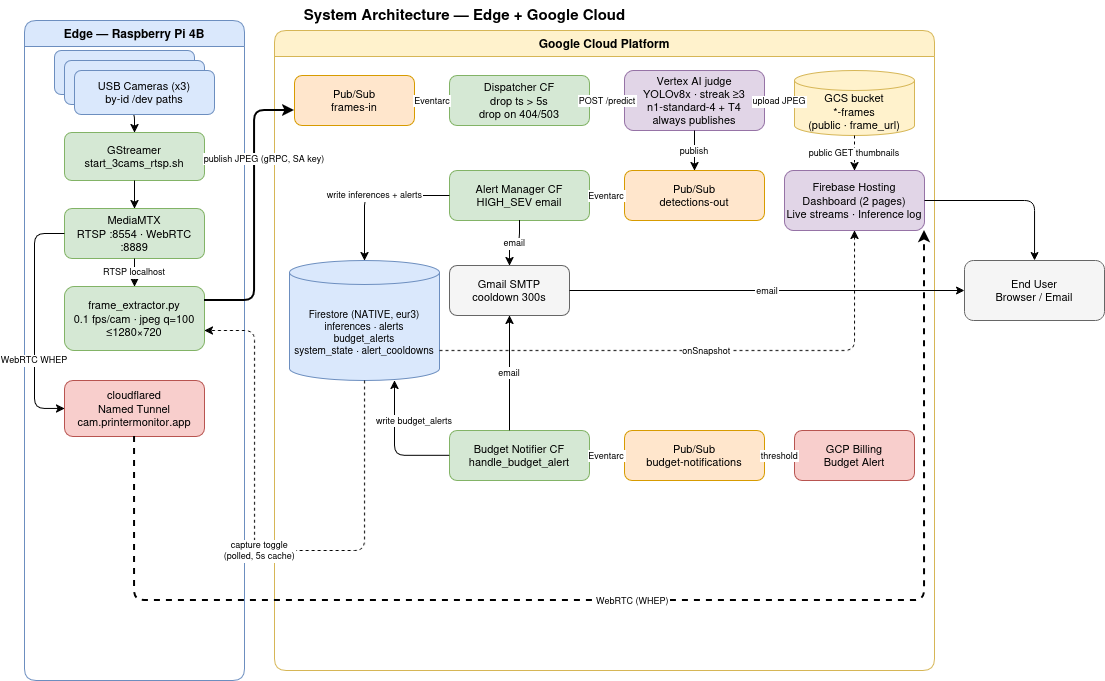
\includegraphics[width=\textwidth]{figures/images/literature/gcp_architecture.drawio.png}}
                    \caption{A rendszer}
                    \label{fig:systemarch}
                \end{figure}


\subsection{Kamera Agent – Raspberry Pi}
    A kamera képek előállításért felelő kamera Agent szerepét egy Raspberry Pi 4B 8GB tölti be,\cite{raspberry_pi}
    3 darab rácsatolt webkamerával kiegészítve. A Raspberry Pi mint edge eszköz rendkívül sokoldalú eszköz.
    Keveset is fogyaszt, megfelelő számú USB porttal is rendelkezik, és az erőforrások is megfelelőek számunkra.
    A Raspberry OS pedig tökéletes a szükséges Docker konténerek és Python szkriptek futtatására.
    


    \section{Szolgáltatások a Pi-n}
    A Pi-n három szolgáltatás fut, melyek az indítás után azonnal elindulnak systemd szolgáltatásként.
    Ezek nélkül a rendszer nem valósulhatna meg.

        \subsection{MediaMTX}
        A MediaMTX (korábban rtsp-simple-server) egy könnyűsúlyú, nyílt forráskódú médiaközvetítő szerver, mely Go programozási nyelven íródott\cite{mediamtx}.
        Szerepe a rendszerben, hogy a webkamerák által előállított nyers videófolyamokat RTSP protokoll szerint tegye elérhetővé a hálózaton.
        A Pi-n systemd szolgáltatásként fut, így az eszköz indításakor automatikusan elindul, emberi beavatkozás nélkül.
        Konfigurációs fájlja definiálja a három kamerastream elérési útját, a kódolási paramétereket, valamint az újracsatlakozási logikát.
        A H264-es kódolású RTSP végpontokat a Cloudflare alagúton keresztül éri el a dashboard, ahol WebRTC formátumban kerülnek megjelenítésre.
        A stream pipeline teljes folyamatát a \ref{fig:mediamtx}. ábra szemlélteti.

        \begin{figure}[H]
            \centering
            {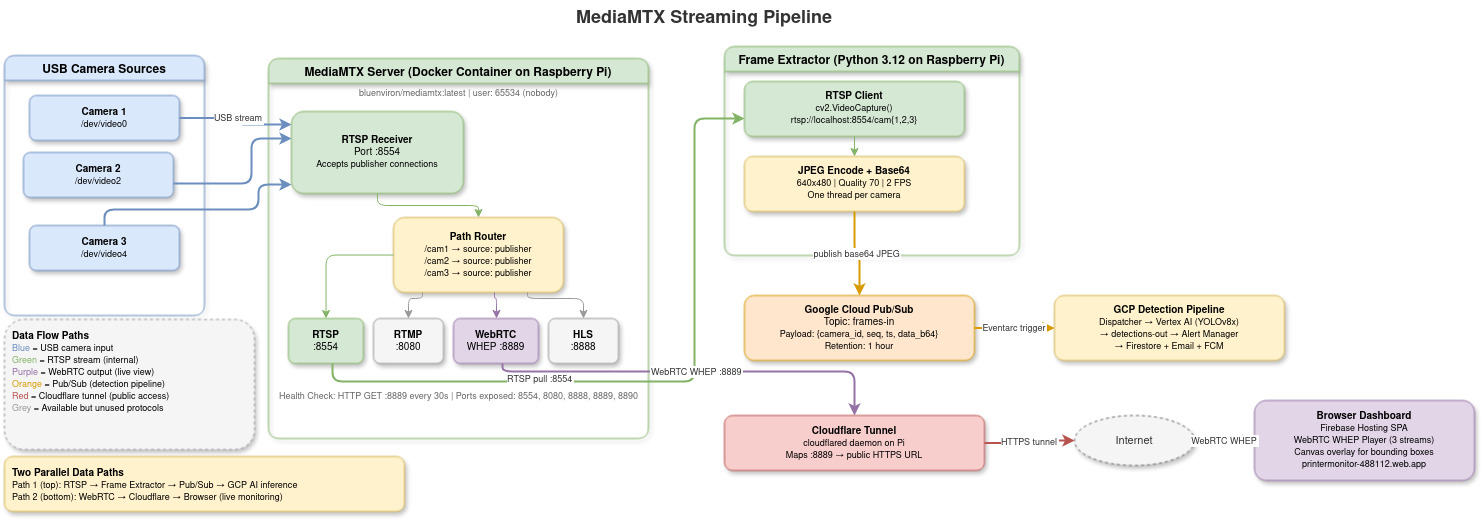
\includegraphics[width=\textwidth]{figures/images/literature/mediamtx_pipeline.jpg}}
            \caption{MediaMTX stream pipeline}
            \label{fig:mediamtx}
        \end{figure}

        \subsection{Képkockák kinyerése}
        A képkockák kinyerésért a \texttt{frame-extractor} szolgáltatás felelős, melynek belépési pontja a \texttt{main.py} Python script.
        Feladata, hogy a három RTSP streamből folyamatosan képkockákat olvasson ki, azokat feldolgozza, majd JSON üzenetként publikálja
        a \texttt{frames-in} Pub/Sub csatornára, ahonnan a \texttt{dispatcher} Cloud Függvény továbbítja őket a Vertex AI végpontra.
        A szolgáltatás a Pi-n systemd szolgáltatásként fut, és az \texttt{sa-frame-extractor} szervízfelhasználó kulcsával hitelesíti magát a Google Cloud felé.

        \subsubsection{Szálkezelés és olvasási modell}
        A script induláskor beolvassa a kamerák RTSP URL-jeit és azonosítóit a környezeti változókból. Minden kamerához két szál tartozik.
        Az első egy folyamatosan futó olvasószál (\texttt{FrameReader}), amely az OpenCV\cite{opencv} \texttt{VideoCapture} osztályán keresztül
        kapcsolódik az adott RTSP streamhez, és a beérkező képkockák közül mindig csak a legfrissebbet tartja meg, a hozzá tartozó,
        a beolvasás pillanatában rögzített UTC-időbélyeggel együtt. Így a publikált képkocka időbélyege a valós rögzítési időpontot tükrözi,
        nem pedig a feldolgozás idejét, ami elengedhetetlen a felhő oldalán végzett elavultság-szűréshez. Ha a kapcsolat megszakad, például
        a kamera újraindul vagy a hálózat elvész, az olvasószál automatikusan újracsatlakozást kísérel meg, így a rendszer emberi beavatkozás nélkül helyreáll.

        \subsubsection{Képfeldolgozás és publikálás}
        A kamerákhoz tartozó második szál a publikáló ciklus (\texttt{publish\_loop}), amely \texttt{CAPTURE\_FPS} ütemben
        (alapértelmezetten 0,1 fps, azaz kameránként tíz másodpercenként egy képkocka) kiveszi az olvasószáltól a legfrissebb képkockát,
        és elvégzi rajta a következő feldolgozási lépéseket:
        \begin{enumerate}
            \item Amennyiben a képkocka mérete meghaladja a konfigurált \texttt{FRAME\_WIDTH} × \texttt{FRAME\_HEIGHT} értéket (alapértelmezetten 1280×720 pixel),
                  az OpenCV a képarány megtartásával lekicsinyíti azt; a célméretnél kisebb képeket változatlanul hagyja.
            \item A képkocka JPEG formátumba kerül kódolásra a beállított \texttt{JPEG\_QUALITY} értékkel (alapértelmezetten 100).
            \item A JPEG bájttömb Base64 kódolással ASCII szöveggé alakul, hogy JSON üzenetbe ágyazható legyen.
            \item A script egy JSON objektumot állít össze, amely tartalmazza a \texttt{camera\_id} azonosítót, a \texttt{seq} szekvenciaszámot,
                  az \texttt{ts} UTC-időbélyeget, valamint a \texttt{data\_b64} mezőt a Base64-kódolt képpel.
            \item A kész JSON payload publikálásra kerül a Pub/Sub \texttt{frames-in} topicra.
        \end{enumerate}
        A publikáló ciklus minden iteráció előtt ellenőrzi a Firestore \texttt{system\_state/extraction} dokumentumának \texttt{enabled} mezőjét
        (öt másodpercre gyorsítótárazva), így a dashboardról szüneteltethető vagy folytatható a képkockák küldése anélkül, hogy a szolgáltatást újra kellene indítani.

        \subsubsection{Health check szerver}
        Mivel a szolgáltatás Cloud Run-kompatibilis konténerként is üzemeltethető, a script egy egyszerű HTTP szervert indít a \texttt{PORT}
        környezeti változóban megadott porton (alapértelmezetten 8080). Ez a szerver minden \texttt{GET} kérésre \texttt{200 OK} választ ad,
        lehetővé téve a platform számára, hogy ellenőrizze a konténer élettartamát.

        \subsubsection{Konfiguráció}
        A script teljes mértékben környezeti változókon keresztül konfigurálható, nem tartalmaz beégetett értékeket.
        A legfontosabb paramétereket az alábbi táblázat foglalja össze:

        \begin{table}[H]
            \centering
            \begin{tabular}{|l|l|l|}
                \hline
                \textbf{Változó} & \textbf{Alapértelmezett} & \textbf{Leírás} \\
                \hline
                \texttt{GCP\_PROJECT}  & - (kötelező) & Google Cloud projekt azonosítója \\
                \texttt{FRAMES\_TOPIC} & - (kötelező) & Pub/Sub topic neve \\
                \texttt{RTSP\_URLS}    & - (kötelező) & Vesszővel elválasztott RTSP URL-ek \\
                \texttt{CAMERA\_IDS}   & cam1,cam2,cam3 & Kamera azonosítók \\
                \texttt{CAPTURE\_FPS}  & 0,1 & Másodpercenkénti képkockák száma \\
                \texttt{JPEG\_QUALITY} & 100 & JPEG tömörítési minőség (0–100) \\
                \texttt{FRAME\_WIDTH}  & 1280 & Képkocka maximális szélessége pixelben \\
                \texttt{FRAME\_HEIGHT} & 720 & Képkocka maximális magassága pixelben \\
                \texttt{PORT}          & 8080 & Health check HTTP szerver portja \\
                \hline
            \end{tabular}
            \caption{A \texttt{frame-extractor} konfigurációs paraméterei}
        \end{table}

        \subsection{Cloudflare alagút}
        A Cloudflare Tunnel egy fordított proxy megoldás, amely lehetővé teszi, hogy a Pi-n futó szolgáltatások nyilvánosan elérhetők legyenek
        anélkül, hogy a routeren portot kellene nyitni, vagy statikus IP-cím szükséges lenne\cite{cloudflare_tunnel}.
        A \texttt{cloudflared} démon a Pi-ről kifelé irányuló titkosított kapcsolatot épít fel a Cloudflare hálózata felé,
        így a tűzfal és a NAT nem akadályozza az elérést. Ez különösen fontos a RTSP videóstreamek dashboardra való eljuttatásakor.

        A Pi-n ez is systemd szolgáltatásként fut, az induláskor automatikusan csatlakozik.
        A rendszer állandó (\textit{named tunnel}) alagutat használ, amely fix, nyilvános aldomainen (\texttt{cam.printermonitor.app}) teszi elérhetővé a streameket.
        Ez a korábban használt ideiglenes (\textit{quick tunnel}) megoldással szemben minden újraindításkor ugyanazt az URL-t tartja meg,
        így a dashboard stream-kapcsolata a Pi újraindítása után sem szakad meg.

    \section{Cloud Stack}
    A rendszer felhőoldali komponensei a Google Cloud Platformon futnak, amely igen széleskörű eszköztárat biztosított a projekt megvalósításához.
    Az infrastruktúra felépítéséhez Terraform keretrendszert használtunk.

        \subsection{Terraform keretrendszer}
        A Terraform egy deklaratív nyelvezetű keretrendszer, mely használatával bármilyen infrastruktúrai elem és erőforrás definiálható
        emberek számára is értelmezhető nyelven\cite{terraform}. Ezen megvalósítások verziózhatóak, disztributálhatóak és bármikor újrafelhasználhatóak.
        Segítségével az alkalmazás minden életszakasza könnyűszerrel menedzselhető, ugyanitt maga az egész folyamat rendkívül könnyen automatizálható.
        
        \subsection{Terraform működése}
        A Terraform a különböző felhőplatformok erőforrásait azok saját API-jain keresztül menedzseli, a közösségnek hála ma már szinte bármelyik
        szolgáltató rendszerét használhatjuk a Terraformon keresztül. Például AWS, Google Cloud, Kubernetes, Git stb. A Terraform működése 3 fázisban történik:

            \subsubsection{Írás-Write}
            Definiáljuk az erőforrásokat, melyek akár több szolgáltatótól is származhatnak, egy .tf kiterjesztésű fileba.
            
            \subsubsection{Tervezés-Plan}
            A \texttt{terraform plan} parancs kiadása után létrejön a terv, mely leírja az infrastruktúrát: mi jön létre, mi változik vagy éppen mi szűnik majd meg.
            Az általunk megadott Konfigurációs fileoknak megfelelően.

            \subsubsection{Alkalmazás-Apply}
            Engedélyezés esetén a Terraform elvégzi a szükséges műveleteket, tiszteletben tartva az erőforrások közötti függőségi sorrendet.
            Létrehozza, módosítja vagy törli az érintett erőforrásokat, majd frissíti az állapotfájlt (\texttt{terraform.tfstate}),
            amely a valós infrastruktúra leképezéseként szolgál a jövőbeli futtatásokhoz.
            A három fázis együttes folyamatát a \ref{fig:terraformstages}. ábra foglalja össze.

                \begin{figure}[H]
                    \centering
                    {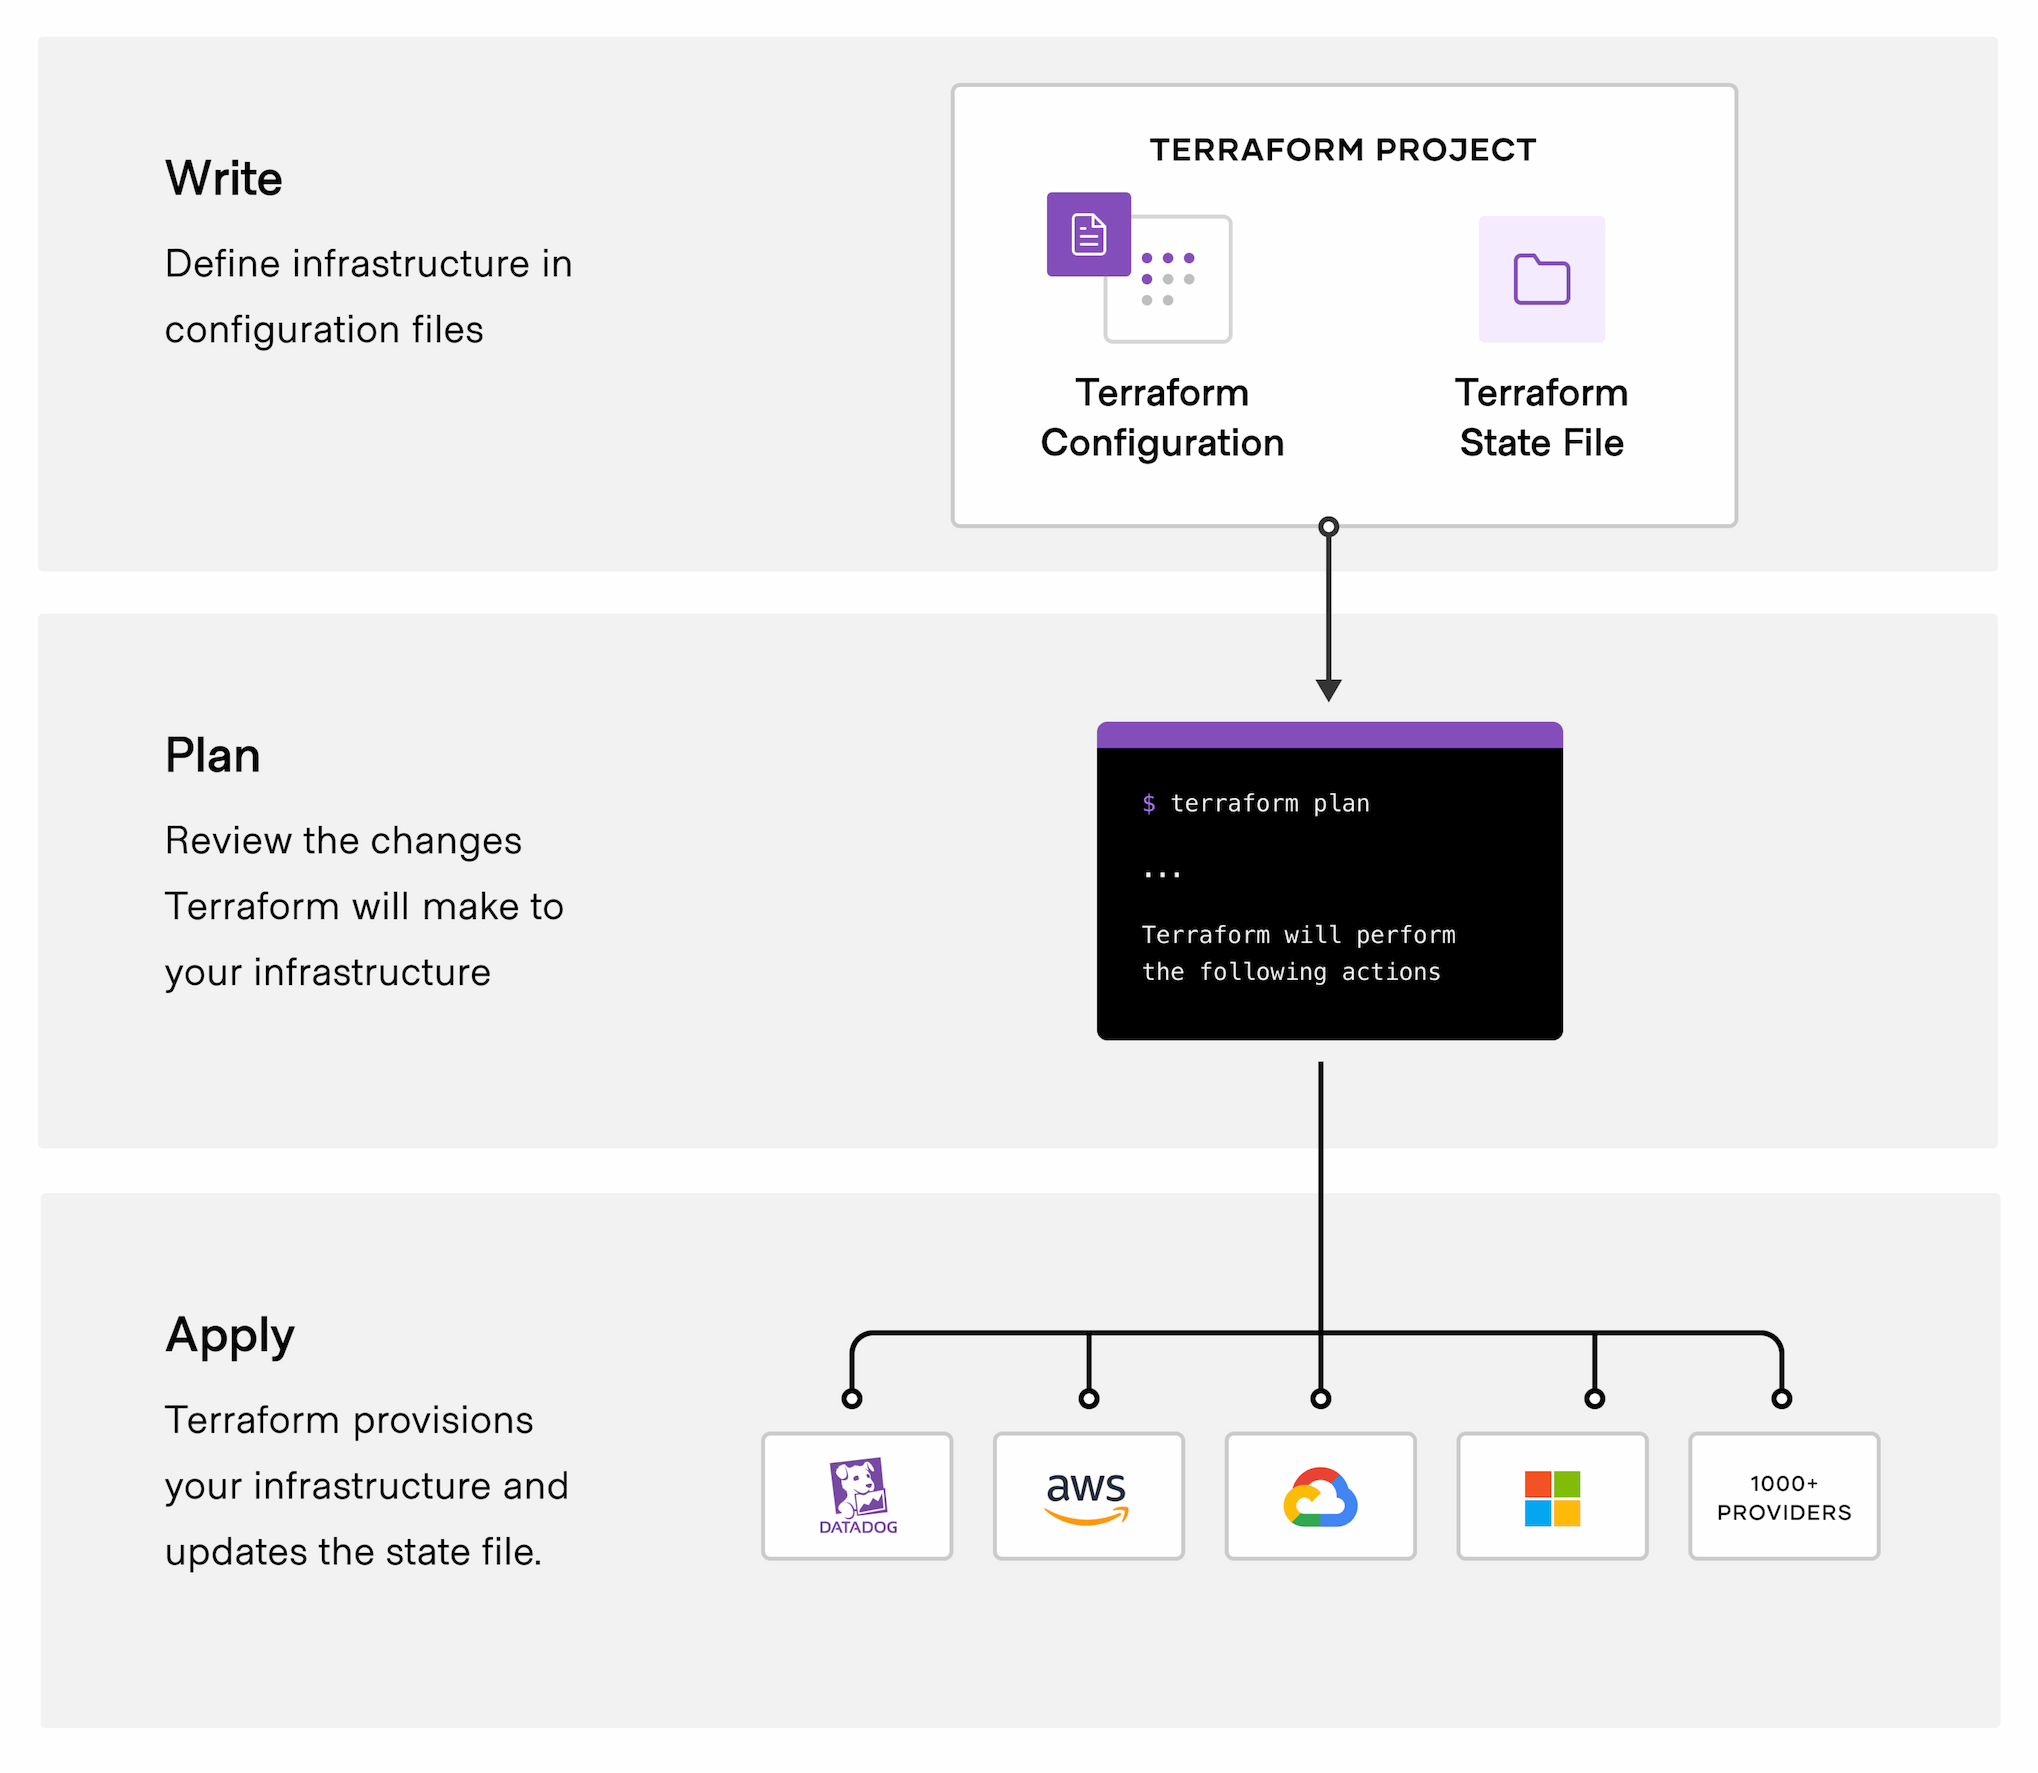
\includegraphics[width=0.6\textwidth]{figures/images/literature/terraformstages.png}}
                    \caption[Terraform Lépések]{Terraform Lépések~\footnotemark}
                    \label{fig:terraformstages}
                \end{figure}
                \footnotetext{\textit{Terraform}: \url{https://developer.hashicorp.com/terraform/intro/}}


        \subsection{Google Cloud Projekt - GCP}
        A rendszer cloud-oldali erőforrásai egyetlen Google Cloud Projektbe szervezett infrastruktúrán futnak, amelynek egyedi azonosítója \texttt{printermonitor-488112}.
        Az összes felhőszolgáltatás, az Artifact Registry-től a Vertex AI végpontig, a Cloud Function-öktől a Firestore adatbázisig, ezen a projekten belül van definiálva és menedzselve.
        A Google Cloud Platform (GCP) választásának fő indoka az volt, hogy egységes ökoszisztémát biztosít a gépi tanulási pipeline-hoz: a Vertex AI natívan integrálódik a Pub/Sub üzenetsorral,
        a Cloud Functions-szel és az Artifact Registry-vel, minimalizálva az integrációs komplexitást\cite{gcp}.
        Az erőforrások számlázása és a költségvetési riasztások szintén ezen a projekten belül vannak konfigurálva, lehetővé téve a kiadások szoros nyomon követését.

        \subsection{Vertex AI végpont}
        A Vertex AI végpont a detekciós pipeline magja: egy egyedi \texttt{judge} Docker konténert futtat, amelyen belül a betanított YOLOv8\cite{yolov8} modell végzi
        a képkockák valós idejű elemzését. A konténer induláskor betölti a modellt a \texttt{MODEL\_PATH} által megjelölt \texttt{best.pt} fájlból,
        majd egy HTTP szerveren (\texttt{/predict} végpont) vár a bejövő kérésekre.

        A szerver kétféle üzenetformátumot kezel: a Vertex AI natív \texttt{\{"instances": [...]\}} formátumát,
        amelyet a Dispatcher Cloud Function küld, valamint a Pub/Sub push formátumát.
        Minden beérkező képkockát Base64-ból visszaalakít, OpenCV-vel dekódol, majd a YOLO modellel elvégzi az objektumdetekciót.
        Az eredmény tartalmazza az észlelt hibaosztályokat (\texttt{label}), azok konfidenciaértékeit, valamint a határoló téglalapok
        koordinátáit mind pixel-, mind normalizált formában.

        A pillanatnyi téves riasztások szűrésére a konténer kameránként és hibaosztályonként számon tartja, hány egymást követő képkockán
        jelent meg ugyanaz a hiba. Egy detekció csak akkor minősül megerősítettnek, ha legalább \texttt{STREAK\_REQUIRED}
        (alapértelmezetten három) egymást követő képkockán át látható; ez kiszűri az egyetlen képkockán felvillanó, zajból eredő észleléseket.
        Mivel ez a számláló a folyamat memóriájában él, a végpontnak egyetlen, állandó példányon (\texttt{min} = \texttt{max} = 1 replika) kell futnia.

        A feldolgozott képkockát a konténer feltölti a \texttt{FRAMES\_BUCKET} névvel megadott GCS tárolóba, és az így kapott nyilvános URL-t a
        \texttt{frame\_url} mezőben csatolja az eredményhez, lehetővé téve, hogy a dashboard utólag a pontosan feldolgozott képet jelenítse meg.
        A detekciós eredmény ezt követően minden képkockára publikálásra kerül a \texttt{detections-out} Pub/Sub csatornára, beleértve azokat is,
        amelyeken nem történt észlelés; erre az adatra a dashboard inferencia-naplója támaszkodik.

        A végpont csak aktív használat közben generál költséget: tétlen (kitelepített, de nem hívott) állapotban nem számlázódik,
        míg folyamatos terhelés esetén napi körülbelül 37\$-os költséggel kell számolni.

        \subsection{Service Accounts}
        A szervíz felhasználók, olyan egyedi emailcímmel rendelkező entitások, melyek segítségével, különböző applikációk, virtuális gépek, vagy egyéb megvalósítások
        kommunikálhatnak a Google API-jával, emberi felhasználók helyett, ezzel biztonságos összeköttetést biztosítva a különböző erőforrások között.

            \subsubsection{sa-frame-extractor}
            \begin{sloppypar}
            A Raspberry Pi-n futó \texttt{frame-extractor} szolgáltatás ezzel a szervízfelhasználóval hitelesíti magát a Google Cloud felé.
            Szerepe, hogy a kinyert képkockák publikálhatóak legyenek a Pub/Sub üzenetbuszra. Jogosultságai: \texttt{pubsub.publisher}
            a \texttt{frames-in} csatornán, valamint \texttt{aiplatform.user} a Vertex AI végpont eléréséhez.
            \end{sloppypar}

            \subsubsection{sa-dispatcher}
            \begin{sloppypar}
            A \texttt{dispatcher} Cloud Function ezzel a szervízfelhasználóval fut. Feladata, hogy a beérkező képkockákat továbbítsa
            a Vertex AI végpontnak, és szükség esetén aktiválja az Alert-Managert. Jogosultságai: \texttt{aiplatform.user} a végpont
            meghívásához, \texttt{pubsub.subscriber} a \texttt{detections-out} csatornán, valamint \texttt{run.invoker} az Alert-Manager
            függvény meghívásához.
            \end{sloppypar}

            \subsubsection{sa-alert-manager}
            \begin{sloppypar}
            A figyelmeztetés kezelésért felelő, egyaránt az anomáliák észlelésekor, és a költségvetés meghaladásakor. Jogosultságai: \texttt{datastore.user},
            \texttt{eventarc.eventReceiver}, \texttt{pubsub.subscriber}, \texttt{run.invoker}.
            \end{sloppypar}

            \subsubsection{sa-cicd}
            \begin{sloppypar}
            A Terraform-infrastruktúra kézi szerkesztése nem ajánlott gyakorlat, ezért ezt egy automatizált GitHub Actions workflow végzi,
            amely ezzel a szervízfelhasználóval hitelesíti magát. Feladata az infrastruktúra kitelepítése és a \texttt{judge} konténer image
            feltöltése. Jogosultságai: \texttt{artifactregistry.writer}, \texttt{pubsub.admin}, \texttt{editor} és \texttt{iam.serviceAccountUser}.
            \end{sloppypar}
            \subsubsection{Vertex AI agent}
            \begin{sloppypar}
            A Vertex AI endpoint a \texttt{judge} (bíró) Docker konténer futtatásáért felelős. Jogosultságai:
            \texttt{pubsub.publisher} a \texttt{detections-out} csatornán.
            \end{sloppypar}

            \subsubsection{Pub/Sub agent}
            \begin{sloppypar}
            A Pub/Sub csatornák menedzselésére szolgál. Jogosultságai: \texttt{iam.serviceAccountTokenCreator}.
            \end{sloppypar}

        \subsection{Pub/Sub Topics}
        A Google Cloud Pub/Sub egy aszinkron üzenetközvetítő szolgáltatás, amely lehetővé teszi az alkalmazáskomponensek közötti laza csatolású kommunikációt\cite{pubsub}.
        A rendszer három darab Pub/Sub csatornát használ, melyek a következők: \texttt{frames-in}, mely a még nyers képkockákat továbbítja a Pi-től a Vertex AI végpont felé.
        A \texttt{detections-out}, mely a Vertex AI végpont által észlelt anomáliák eredményét továbbítja a dashboard felé, és a \texttt{budget-notifications}, mely figyelmeztet minket
        amennyiben átléptük a kiszabott költségvetést.
            
                

        \subsection{Google Cloud Függvények}
        A rendszer három Cloud Function (Gen2) példányt alkalmaz, amelyek Pub/Sub eseményekre triggerelődnek és kiszolgáltatás nélkül,
        skálázhatóan futnak. Mindhárom függvény az \texttt{sa-alert-manager}, illetve \texttt{sa-dispatcher} szervízfelhasználó jogosultságaival rendelkezik.

            \subsubsection{Dispatcher}
            A Dispatcher hidat képez az edge eszköz és a Vertex AI végpont között. A \texttt{frames-in} Pub/Sub csatornáról kap üzenetet,
            amelynek tartalma egy Base64-kódolt JPEG képkocka, a kamera azonosítója, egy szekvenciaszám és egy UTC időbélyeg.
            A függvény ezt az adatot a Vertex AI REST API-jára továbbítja (\texttt{/predict} végpont), OAuth2 Bearer tokennel hitelesítve.
            Ha a Vertex AI kérés hálózati hiba miatt meghiúsul, a függvény újra dobja a kivételt, így a Pub/Sub automatikusan újrapróbálkozik.
            A három Cloud Függvény közül ez a leginkább memóriaigényes, mivel képkockák bináris adatát szállítja HTTP-n keresztül.

            \subsubsection{Alert-Manager}
            A detekciós pipeline záró állomása. A \texttt{detections-out} csatornáról érkező minden üzenetet, a hiba nélkülieket is,
            naplóz a Firestore \texttt{inferences} kollekciójába, amely a dashboard inferencia-naplójának forrása. Ezt követően kiszűri azokat
            a detektált hibákat, amelyek konfidenciaértéke eléri a beállított küszöböt (alapértelmezetten 35\%). Az átmenő detektálásokat a Firestore
            \texttt{alerts} kollekcióba írja, rögzítve a kamera azonosítóját, az észlelt hibákat, az időbélyeget és a szekvenciaszámot.

            E-mail értesítést kizárólag magas súlyosságú hibaosztályok esetén küld: \texttt{spagetti}, \texttt{not\_sticking},
            \texttt{layer\_shift} és \texttt{warping}. Az ismétlődő riasztások elkerülése érdekében egyetlen, az egész rendszerre közös,
            300 másodperces visszatartási időt (\textit{cooldown}) alkalmaz, amelyet a Firestore \texttt{alert\_cooldowns} kollekciójában,
            a \texttt{global\_email} kulcs alatt tárol. A visszatartás csak akkor indul el, ha az e-mail ténylegesen kiment, így egy átmeneti
            SMTP-hiba nem nyomja el a következő riasztást. Az e-mail HTML formátumú, tartalmazza az észlelt hibák táblázatát és egy közvetlen linket a dashboardra.

            \subsubsection{Budget Notifier}
            E függvény célja, hogy megakadályozza a felhőköltségek elszabadulását. A \texttt{budget-notifications} Pub/Sub csatornán
            hallgatózik, amelyre a GCP saját költségvetési riasztó rendszere publikál, ha az előre beállított kiadási küszöb teljesül.
            A függvény az Alert-Managerrel közös kódbázisban van megvalósítva, és szintén cooldown mechanizmust alkalmaz.
            Az eseményt a Firestore \texttt{budget\_alerts} kollekcióba is naplózza, majd HTML e-mailben értesíti a felhasználót
            a felhasznált összegről és a küszöbértékről.

            
        \subsection{Firestore Collections}
        Az adatbáziskezelő rendszereknek két nagy fajtáját különböztetünk meg, a relációs adatbázisokat, és a nem relációs avagy NoSQL (Not only SQL) adatbázisokat.
        A fő különbség, hogy a relációs adatbázisokban az adatok táblákba rendezettek, és köztük jól meghatározott kapcsolatok vannak. Viszont a NoSQL adatbázisokban az
        adatok úgynevezett dokumentumokban vannak eltárolva, melyek szerkezete sokkal rugalmasabb és nem igényel előre meghatározott sémát. Mivel a projekt főként JSON formátumú
        adatokkal dolgozik, így a NoSQL adatbázisok sokkal jobban megfelelnek a céljainknak, és a Firestore egy igen népszerű és megbízható választás ezen a téren\cite{firestore}.

        A rendszer az alábbi Firestore kollekciókat és állapotdokumentumokat használja:

        \begin{itemize}
            \item Az \texttt{inferences} kollekció minden egyes feldolgozott képkocka inferencia-eredményét tárolja, a hiba nélkülieket is.
            Ez a kollekció szolgál a dashboard inferencia-naplójának adatforrásául, és a hozzá tartozó \texttt{frame\_url} mezőn keresztül
            a pontosan feldolgozott képkocka is visszanézhető.

            \item Az \texttt{alerts} kollekció tárolja a detektált anomáliák bejegyzéseit. Mezői: \texttt{camera\_id} (melyik kamera észlelte),
            \texttt{detections[]} (a hibák tömbje: név + konfidencia + bounding box), \texttt{timestamp} (mikor történt a detekció),
            \texttt{seq} (a képkocka szekvenciaszáma, amelyet a \texttt{frame-extractor} biztosít) és \texttt{created\_at} (mikor került be a bejegyzés).
            A dashboardon való hatékony keresést egy kompozit index segíti: \texttt{camera\_id ASC} + \texttt{timestamp DESC},
            azaz kamera szerint növekvő, időbélyeg szerint csökkenő sorrendben.

            \item Az \texttt{alert\_cooldowns} kollekció az e-mail értesítések visszatartási idejét kezeli. Egyetlen, az egész rendszerre közös
            \texttt{global\_email} kulcs alatt tárolja a legutóbbi sikeres küldés időpontját, megakadályozva a riasztás-özönt rövid időn belül ismétlődő anomáliák esetén.

            \item A \texttt{budget\_alerts} kollekció a GCP költségvetési riasztásokat naplózza, beleértve a felhasznált összeget,
            a beállított küszöböt és az esemény időbélyegét.

            \item A \texttt{system\_state/extraction} dokumentum tárolja a képkocka-rögzítés be- vagy kikapcsolt állapotát (\texttt{enabled} mező).
            A dashboardról az operátor állítja, a Raspberry Pi-n futó \texttt{frame-extractor} pedig ezt olvassa, így a rögzítés távolról szüneteltethető.
        \end{itemize}


        \subsection{Konténer képek}
        A Vertex AI végponton futó detekciós logika egy egyedi Docker konténer képbe (image) van csomagolva, melynek neve \texttt{judge}.
        Ez az image egy Python scriptet tartalmaz, amely induláskor betölti a betanított YOLOv8 modellt, majd várakozik a bejövő Pub/Sub üzenetekre.
        Egy üzenet érkezésekor kicsomagolja a base64-kódolt JPEG képkockát, elvégzi rajta az objektumdetekciót, majd az eredményt, a detektált hibaosztályokat és azok konfidenciaértékeit,
        visszapublikálja a \texttt{detections-out} Pub/Sub csatornára\cite{vertexai_custom_container}.
        Az image tárolása a Google Artifact Registry-ben történik, verziózva a commit SHA alapján.
        Minden módosítás esetén a \texttt{docker-judge.yml} GitHub Action automatikusan újrabuildi és feltölti a friss image-t, ahonnan a Vertex AI végpont azt lehúzza és futtatja.
        A konténer teljes életciklusát, a build fázistól a futtatásig, a \ref{fig:judge}. ábra mutatja be.

        \begin{figure}[H]
            \centering
            {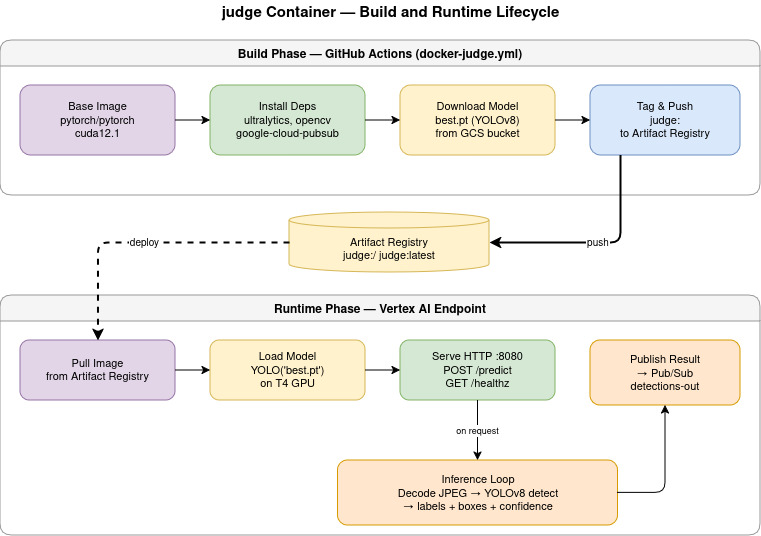
\includegraphics[width=\textwidth]{figures/images/literature/judge_cicd_pipeline.jpg}}
            \caption{A \texttt{judge} konténer image életciklusa}
            \label{fig:judge}
        \end{figure}

    \section{Dashboard}
    A rendszer felhasználói felülete egy webalkalmazás, melyet a Firebase Hosting platform szolgál ki,
    így külön szerver üzemeltetése nélkül érhető el a böngészőből\cite{firebase_hosting}. A felület két nézetből áll.

    Az első nézet (\textit{Live streams}) valós időben jeleníti meg a három kamera videofolyamát WebRTC technológia segítségével,
    a MediaMTX szerveren és a Cloudflare alagúton keresztül érkező RTSP streamekre támaszkodva. Erre a nézetre a Firebase Firestore
    adatbázishoz való közvetlen, valós idejű kapcsolaton keresztül (\texttt{onSnapshot} listener) kerülnek rá a nemrég megerősített
    detekciók jelölései; ezek néhány tíz másodperces késéssel követik az élő képet, mivel előbb végig kell haladniuk a teljes feldolgozási láncon.
    Ugyanitt található a rögzítés be- és kikapcsolására szolgáló vezérlő is, amelyet csak operátori Google-fiókkal bejelentkezve lehet
    használni; ez a \texttt{system\_state/extraction} dokumentumot írja, amelyet a Raspberry Pi olvas.

    A második nézet (\textit{Inference log}) az \texttt{inferences} kollekcióból építkezik: minden feldolgozott képkockához megjeleníti
    a hozzá tartozó képkocka-bélyeget és a detekciók táblázatát, a határoló téglalapokat pedig pontosan arra a képkockára rajzolja,
    amelyet a modell ténylegesen feldolgozott. Így ez a nézet képkocka-szinten hű képet ad a modell döntéseiről.

    A dashboard vizuálisan is visszajelzést ad a rendszer állapotáról: normál működés közben a felület semleges állapotot mutat
    (\ref{fig:dash_normal}. ábra), amennyiben pedig magas prioritású anomália érkezik, a felület piros kerettel jelenik meg
    (CSS \texttt{alerting} osztály aktiválásával), ahogy azt a \ref{fig:dash_high}. ábra szemlélteti.
    Hasonlóan, a költségvetési riasztás esetén sárga kerettel jelez (\texttt{budget-alert} osztály),
    így a felhasználó azonnal értesül a túllépésről anélkül, hogy az e-mailjét kellene ellenőriznie.

    \begin{figure}[H]
        \centering
        {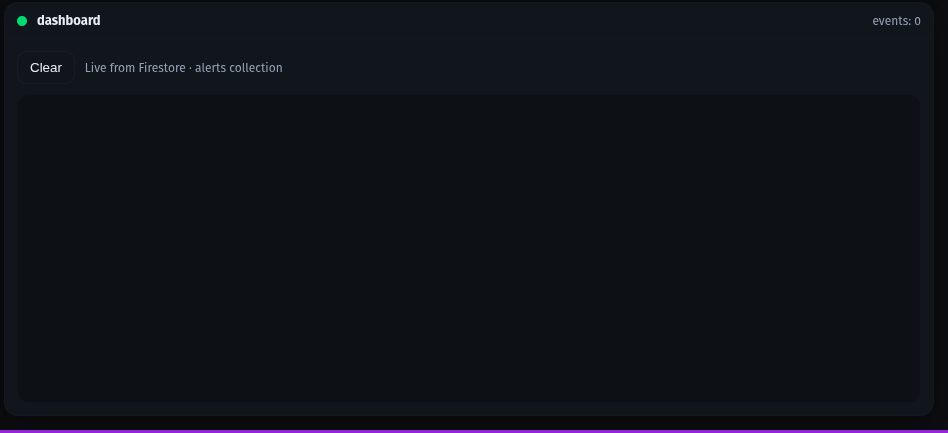
\includegraphics[width=\textwidth]{figures/images/literature/dash_normal.png}}
        \caption{A dashboard normál működési állapotban}
        \label{fig:dash_normal}
    \end{figure}

    \begin{figure}[H]
        \centering
        {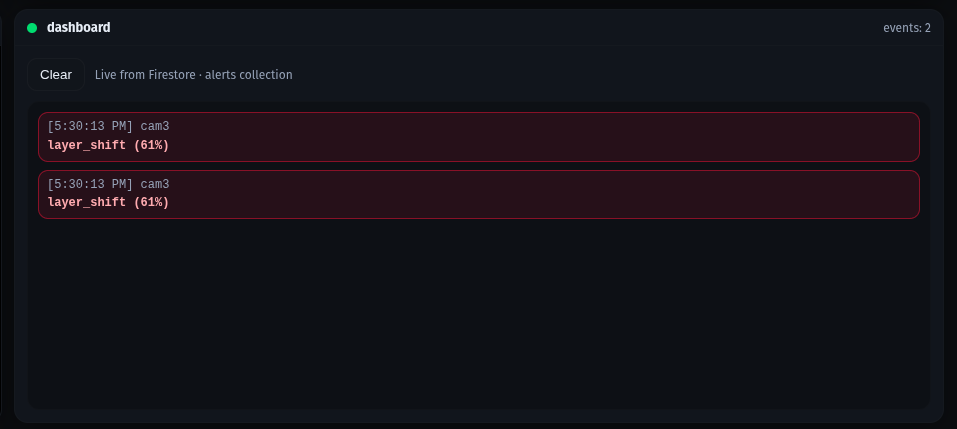
\includegraphics[width=\textwidth]{figures/images/literature/dash_high.png}}
        \caption{A dashboard anomália detektálás esetén}
        \label{fig:dash_high}
    \end{figure}

    \section{GitHub Action Workflows}
    A projekt folyamatos integrációját és automatizált kitelepítését (CI/CD) több GitHub Action workflow biztosítja,
    melyek a megfelelő kódváltozásra automatikusan lefutnak, csökkentve a manuális beavatkozás szükségességét és az emberi hibák esélyét\cite{github_actions}.
    Az infrastruktúra és a konténer kezelésén túl egy külön workflow (\texttt{python-tests.yml}) minden, a szolgáltatások kódját érintő változásnál
    lefuttatja a Python egységteszteket, és 90\%-os lefedettségi küszöböt vár el, egy további workflow (\texttt{compileLatex.yml}) pedig a dolgozat
    PDF-jét fordítja újra. Az alábbiakban a két fő, infrastruktúrát és konténert érintő workflow-t mutatjuk be részletesen.

        \subsection{Terraform lépések automatizálása}
        Ez a workflow a felhőinfrastruktúra változtatásait kezeli automatikusan.
        Pull request esetén csak ellenőrző lépések futnak le, hogy a változtatások biztonságosak és helyesek legyenek a merge előtt:
        a workflow lefuttatja a \texttt{terraform plan} parancsot, amelynek kimenetét egy emberi felülvizsgáló a pull request keretében
        ellenőrzi, mielőtt jóváhagyná az összevonást. Merge eseményre a \texttt{main} ágra a workflow elvégzi a tényleges infrastruktúra
        módosítást (\texttt{terraform apply}) a GCP-n.

        Megjegyzendő korlát, hogy a tervet (\texttt{plan}) és annak alkalmazását (\texttt{apply}) jelenleg a merge eseménye kapcsolja össze:
        a \texttt{main} ágra történő összevonás után az \texttt{apply} külön emberi megerősítés nélkül lefut. Robusztusabb megoldás lenne
        egy explicit, kézi jóváhagyási kapu (\textit{manual approval gate}) beiktatása közvetlenül az \texttt{apply} lépés elé, amely a
        ténylegesen alkalmazandó tervet még egyszer felülvizsgálatra bocsátja; ez a jövőbeli fejlesztések egyik iránya.

            \subsubsection{Konfigurációs ellenőrzés – Checkov}
            A Checkov egy nyílt forráskódú statikus elemző eszköz, amely Terraform konfigurációkat vizsgál ismert biztonsági problémák és rossz praktikák szempontjából\cite{checkov}.
            Futtatása pull request esetén kötelező lépés: amennyiben magas súlyosságú problémát talál, például nyilvánosan elérhető storage bucket vagy nem megfelelő IAM konfiguráció,
            a workflow megakadályozza a merge-t. Ez biztosítja, hogy a fejlesztés során se kerülhessen sérülékeny infrastruktúra a produkcióba.

            \subsubsection{Formázás és erőforráshasználat ellenőrzés-Lint}
            A linting lépés két dolgot ellenőriz. A \texttt{terraform fmt --check} parancs megvizsgálja, hogy a \texttt{.tf} fájlok formázása megfelel-e a Terraform hivatalos stílusirányelveknek.
            A \texttt{terraform validate} parancs pedig szintaktikailag és szemantikailag ellenőrzi a konfigurációt, kiszűrve a nem létező erőforrásokra való hivatkozásokat
            vagy érvénytelen argumentumokat. Ezzel a lépéssel a triviális hibák már a review fázisban kiszűrhetők.

        \subsection{Docker konténer felépítésének automatizálása}
        Ez a workflow a \texttt{judge} Docker image buildjeléért és az Artifact Registry-be való automatikus feltöltéséért felelős.
        Minden olyan push eseményre lefut, amely a \texttt{judge/} könyvtárat érinti, így csak releváns változtatás esetén indul el, nem feleslegesen.
        A workflow lépései sorban: hitelesítés az \texttt{sa-cicd} service account kulcsával, az image buildje, ellátása a commit SHA-val mint egyedi taggel,
        majd feltöltése a Google Artifact Registry-be. Ezt követően a Vertex AI végpont a következő aktiváláskor automatikusan az új image-t fogja használni.
        A két workflow együttes működését a \ref{fig:cicd}. ábra foglalja össze.

        \begin{figure}[H]
            \centering
            {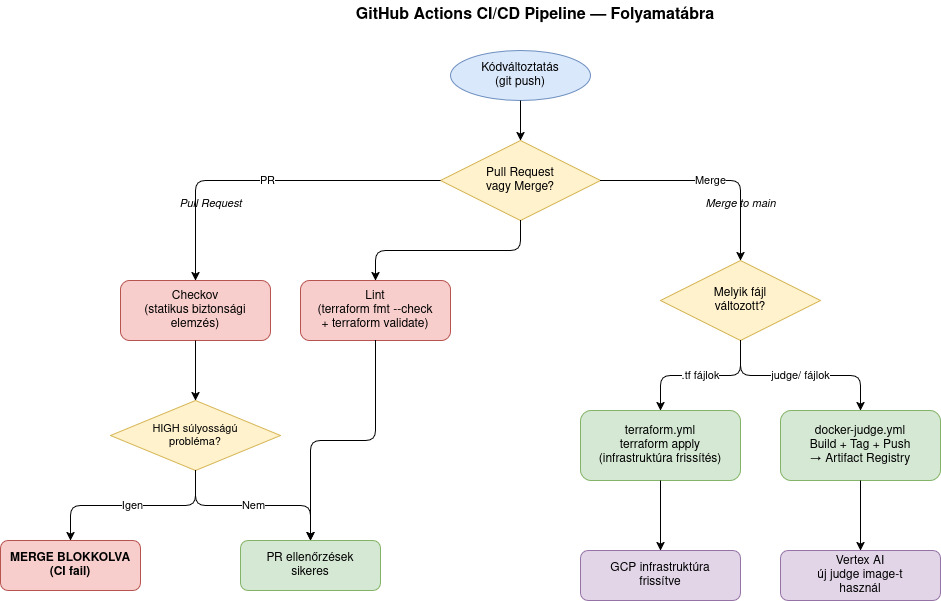
\includegraphics[width=\textwidth]{figures/images/literature/github_actions_cicd.jpg}}
            \caption{A CI/CD pipeline lépései}
            \label{fig:cicd}
        \end{figure}

    \section{Összefoglalás}
    A fejezet bemutatta a rendszer teljes hardver- és szoftverkörnyezetét.
    Az edge oldalon egy Raspberry Pi 4B gondoskodik a kameraképek rögzítéséről és valós idejű továbbításáról,
    a felhő oldalon pedig a Google Cloud Platform szolgáltatásai, Pub/Sub, Cloud Functions, Vertex AI, Firestore és Firebase Hosting,
    alkotják azt a pipeline-t, amely a nyers képkockáktól az anomáliadetekción át a felhasználói értesítésig minden lépést lefed.
    Az infrastruktúra Terraformmal van definiálva és verziókezelve, a CI/CD pipeline pedig biztosítja,
    hogy minden kódváltozás automatikusan, emberi beavatkozás nélkül jusson el az éles környezetbe.
